\immediate\write18{bibtex \jobname}
\documentclass{amsart}
\usepackage{amsmath, amsthm, amssymb}
\usepackage[colorlinks=true,linkcolor=blue,urlcolor=blue]{hyperref}
\usepackage[capitalize,noabbrev]{cleveref}
\usepackage{tikz-cd}
%\usepackage{newtxtext,newtxmath}
\usepackage[numbers,sort,compress]{natbib}
\usepackage{graphicx}

%To-do
\usepackage[marginpar]{todo}
\makeatletter
\renewcommand{\@tododisplay}[1]{%
%\marginpar{#1}%
\textsuperscript{#1}%
}
%
\renewcommand\@displaytodo[2][\todomark]{%
\@tododisplay{{\todoformat [#1~\ref{todolbl:\thetodo}]}}%
\footnotetext[\thetodo]{\todoformat #1:~#2}%
\global\@todotoks\expandafter{\the\@todotoks\todoitem{#1}{#2}}%
\@todotrue%
}%
\renewcommand\todomark{todo}
\makeatother

% theorems
\theoremstyle{plain}
\newtheorem{thm}{Theorem}[section]
\Crefname{thm}{Theorem}{Theorems}
\newtheorem{cor}[thm]{Corollary}
\newtheorem{lem}[thm]{Lemma}
\newtheorem{prop}[thm]{Proposition}
\Crefname{prop}{Proposition}{Propositions}
\newtheorem{claim}[thm]{Claim}
\newtheorem{conj}[thm]{Conjecture}
\Crefname{conj}{Conjecture}{Conjectures}
\theoremstyle{definition}
\newtheorem{defi}[thm]{Definition}
\newtheorem{ex}[thm]{Example}
\newtheorem{rem}[thm]{Remark}

% commands
\newcommand{\N}{\mathbb{N}}
\newcommand{\Z}{\mathbb{Z}}
\newcommand{\R}{\mathbb{R}}
\newcommand{\HS}{\mathrm{HS}}
\newcommand{\HT}{\mathrm{HT}}
\newcommand{\HLC}{\mathrm{HLC}}
\renewcommand{\H}{\mathbb{H}^d}
\newcommand{\dprime}{{\prime\prime}}
\DeclareMathOperator{\interior}{int}
\DeclareMathOperator{\im}{im}
\newcommand\CH{\check{H}}

% margins
\setlength{\textwidth}{\paperwidth}
\addtolength{\textwidth}{-1.6in}
\setlength{\textheight}{\paperheight}
\addtolength{\textheight}{-1.8in}
\calclayout

\newcommand{\anibal}[1]{\textcolor{blue}{[Anibal: #1]}}

\begin{document}

\title[Persistence in functional topology]{Persistence in functional topology: q-tameness, local-connectivity and a correction to a theorem of Morse}
\author{}
\date{\today}

\begin{abstract}
With applications to the study of minimal surfaces in mind, Marston Morse wrote a series of papers developing versions of his famous inequalities for a broad class of real-valued functions on metric spaces. His work is remarkable in so far as it likely represents the first use of something that can be called persistent homology in the mathematical literature. From the modern point of view, it is particularly interesting that he uses Vietoris homology in order to enforce semi-continuity of persistent homology and that he states two topological conditions that supposedly ensure q-tameness. However, he is partly incorrect: We present a filtration that satisfies one of his conditions but has non-q-tame persistent homology. We also conjecture that his other condition, for which he provides no proof, is correct and discuss possible proof strategies.
\end{abstract}

\maketitle


\section{Introduction}

The interplay between the critical set of a function and the topology of its domain is a cornerstone of modern mathematics.
Nowadays, when thinking about the pioneering work of Marston Morse, our first thought probably involves a differentiable function on a closed smooth manifold, but more general settings should also be considered.
Morse theory in the smooth context was masterfully presented in Milnor's famous book on the subject \cite{Milnor.1963}, where he also gave a new proof of Bott's periodicity by applying Morse theory to the energy functional of paths in a Riemannian manifold, which notably goes beyond the compact setting.
Another important example of the use of Morse's insights in an infinite context is Floer's work on the Arnold conjecture and its many ramifications in symplectic topology, as surveyed for example in \cite{Salamon.1999}.
Morse himself worked in a very general setting, publishing in the 1930s a pair of papers \cite{Morse.1937, Morse.1940} and a monograph \cite{Morse.1938} in which he established the key results of Morse theory in the broad context defined by semi-continuous functionals on metric spaces.
He called the theory set forth in this body of work \emph{functional topology} and used it to study questions about minimal surfaces motivated by Douglas' solution to Plateau’s Problem \cite{Douglas.1931}.
In particular, Morse and Tompkins \cite{Morse.1939, Morse.1941} used these techniques to prove a general form of \emph{Mountain Pass Theorem} --~an existence result for saddle points~-- applying to functions that are not necessarily continuous.
From this, they deduce their \emph{Unstable Minimal Surface Theorem}, showing the existence of critical points of the Douglas functional that are not local minima.

Morse's work on functional topology did not have a long lasting impact on minimal surface theory or the calculus of variations in general; possibly in part because, as expressed by Struwe:
\begin{displaycquote}[p.~82]{Struwe.1988}
	The technical complexity and the use of a sophisticated topological machinery [...] tend to make Morse--Tompkins' original paper unreadable and inaccessible for the non-specialist.
\end{displaycquote}
A similar assessment was given by Raoul Bott, who writes in \cite[p.~934]{Bott.1980} that the papers \cite{Morse.1937, Morse.1940} ``are not easy reading'' and constitute a ``tour de force'' by Morse.

The intricacies of Morse's development notwithstanding, many of his ideas have resurfaced in the intervening years and flourished in other domains.
In particular, in applied topology and topological data analysis, several key insights of Morse have been independently rediscovered as part of the development of \emph{persistent homology}, a technique that provides robust and efficiently computable invariants of filtered spaces using the functorial properties of homology.
Its success in applied topology has motivated a refined abstract theory of persistence that lies in the intersection of geometry, topology, and representation theory.

The homology of a filtered space is an example of what is called a \emph{persistence module}, a functor to vector spaces from the real numbers considered as a poset category.
In many important cases, a persistence module $M$ admits an essentially unique decomposition into indecomposable direct summands, and the structure of this decomposition yields a complete discrete invariant of $M$ known as its \emph{persistence diagram}.
The set of all persistence diagrams can be organized into a metric space.
This often allows to recast geometric questions about general filtered spaces in a combinatorial metric model, since the passage via the homology construction to this metric space is Lipschitz, a statement commonly known as the \emph{stability} of persistence diagrams.

The most remarkable connections between functional topology and persistence theory come from Morse's paper \cite{Morse.1940}, where he developed the theory of \emph{caps} and their \emph{spans}.
They capture much of the same information as the modern notion of persistence diagram, including concepts such as the persistence or birth and death of a homology class, although Morse's results still fall short of yielding global decompositions of persistence modules.
Morse used his theory of caps to study functionals on a metric space by analyzing the evolution of the topology of their sublevel sets.
A key tool for this end is a version of his eponymous inequalities for cap numbers, which expands their usual version in the compact and smooth setting.
In this work, using persistence diagrams, we generalize the definition of these cap numbers to persistence modules and prove the existence of Morse inequalities for a large class of them (\cref{t:inequalities}).
Our approach makes these inequalities accessible in new contexts beyond those originally covered by functional topology, including, for example, symplectic geometry.

Given the importance of persistence diagrams for stating and proving Morse inequalities, our focus will then be on the study of topological properties ensuring their existence for a broad class of filtered spaces and homology constructions.
For general persistence modules, a well studied condition for the existence of persistence diagrams is \emph{q-tameness} \cite{Chazal.2016a,Chazal.2016b}, which simply states that all linear maps between different real values in the persistence module have finite dimensional rank.
The motivating question can then be reformulated as asking for topological conditions on a filtered space that ensure its persistent homology to be q-tame.
In fact, the problem of finding such conditions was already considered by Morse, who studied certain local connectivity properties of a filtered metric space and claimed them to suffice for the q-tameness of the associated persistent \v{C}ech homology.
Contrary to these claims, we show that the local connectivity condition used by Morse and Tompkins in the proof of the Unstable Minimal Surface Theorem is insufficient (\cref{c:counterexample}).
We introduce two similar but more widely applicable conditions, and show that the first suffices for the \mbox{q-tameness} of filtrations defined by continuous functionals (\cref{c:q-tameness for continuous functions}), and the second for those defined by functionals with compact sublevel sets (\cref{t:local connectedness implies q-tameness}).
Since Douglas' functional has compact sublevel sets but is not continuous in the $C^0$ topology considered by Morse and Tompkins, we use this second condition to correct their proof.

\subsection*{Summary}

The primary contribution of this work consists in the introduction of topological conditions on a broad class of filtered spaces ensuring their associated persistent homology modules satisfy Morse inequalities.
As an application of our results, we identify and fix a mistake in the proof the Unstable Minimal Surface Theorem of Morse and Tompkins.

\subsection*{Outline}

In \cref{s:persistence} we recall the foundations of persistence theory where, for us, the persistent homology of a sublevel set filtration is the key example.
We present a persistence-theoretic point of view on Morse inequalities in \cref{s:inequalities}.
It generalizes both their versions in the smooth and compact setting as well as the one used in functional topology.
The core of this work is presented in \cref{s:connectivity}, where we define two natural notions of local-connectivity for a sublevel set filtration and show under what circumstances they imply q-tameness for its associated persistence module.
We close in \cref{s:surfaces} with a historical overview of Morse--Tompkins' use of functional topology in minimal surface theory, and explore its relation to our results.
\cref{s:vietoris} contains a brief discussion on the definitions of Vietoris and \v{C}ech homology and a comparison between them based on Dowker's Theorem.

\section{Preliminaries}

\begin{itemize}
	\item metric space
	\item upper semi-continuous function
	\item Persistence module
	\item q-tameness
	\item Barcode
	\item bottleneck
	\item stability
\end{itemize}

\begin{defi}
	Let $M$ be a metric space. For any $p \in M$ and $\epsilon \geq 0$ denote
	\begin{equation*}
	B_\epsilon(p) = \{q \in M\ |\ d(p,q) < \epsilon\}, \qquad
	\overline B_\epsilon(p) = \{q \in M\ |\ d(p,q) \leq \epsilon\}.
	\end{equation*}
\end{defi}

\begin{defi}
	Let $X$ be a space and $f \colon X \to \R$ a function. For any $t \in \R$, the \textit{$t$-sublevel set of $f$} is defined by 
	\begin{equation*}
	X_{\leq t} = f^{-1}((-\infty, t]).
	\end{equation*}
\end{defi}

\section{Persistence diagrams from local connectivity} \label{s:connectivity}

We have seen that q-tame functions admit persistence diagrams, which can be used to formulate Morse inequalities.
With q-tameness being a rather abstract condition, we now establish more concrete topological conditions that ensure the q-tameness of a function.
Our definitions are motivated by similar conditions that Morse considered in his work on functional topology.
We will present a historical account in \cref{s:surfaces}.

Whether a function is q-tame or not depends on the functor that is used to pass from the sublevel set filtration of the function to a persistence module.
The general idea that we want to employ is to deduce global finiteness properties like q-tameness from local ones.
Thus, the functors we consider should have some property that allows us to do so.

Concretely, let $\H = (\H_d)_{d \in \Z} \colon \Top \to \Vect$ be a fixed graded homotopy invariant functor, which we call a \emph{homology theory}.
A triple of spaces $X_{1}, X_{2} \subseteq X$ is said to have a \emph{Mayer-Vietoris sequence} for $\H$ if the inclusion-induced maps fit in a long exact sequence
\begin{equation*}
\begin{tikzcd}[column sep = small]
\cdots \arrow[r] & \H_{n}(X_{1} \cap X_{2}) \arrow[r] & \H_{n}(X_{1}) \oplus \H_{n}(X_{2}) \arrow[r] & \H_{n}(X) \arrow[r] & \H_{n-1}(X_{1} \cap X_{2}) \arrow[r] & \cdots \ .
\end{tikzcd}
\end{equation*}
We say that $\H$ has the \emph{open} (resp.\@\  \emph{compact}) \emph{Mayer-Vietories property} if there are natural Mayer-Vietoris sequences for all triples $X_{1}, X_{2} \subseteq X$ with $X = X_1 \cup X_2$ and $X_i \subseteq X$ open (resp.\@\ compact Hausdorff).

For the rest of this section, we will assume that $\H$ is a homology theory that has either the open or the compact Mayer-Vietoris property and for which there is $n_0$ such that $\H_{n}$ is 0 for all $n \leq n_0$.
Note that this includes singular homology with field coefficients, which, like any homology theory in the sense of the Eilenberg-Steenrod axioms \cite[Section I]{MR0050886}, has the open Mayer-Vietoris property, and it also includes \v{C}ech homology with field coefficients, which has the closed Mayer-Vietoris property.

\begin{defi} \label{defi:local_connectedness}
	For $n \in \Z$ a continuous map is said to be \textit{$n$-homologically small} or $\HS_n$ if the image of the map induced by $\H_{n}$ is finite dimensional.
	We omit references to $n$ if the condition holds for all integers.
\end{defi}

\begin{defi} \label{defi:local_connectedness_filtrations}
	The sublevel set filtration of a function $f \colon X \to \R$ is said to be \emph{locally homologically small} or $\HLC$ if for any $x \in X$, any neighborhood $V$ of $x$, and any index $t > f(x)$, there is an index $s$ with  $f(x) < s < t$ and a neighborhood $U$ of $x$ with $U \subseteq V$ such that the inclusion $f_{\leq s} \cap U \to f_{\leq t} \cap V$ is $\HS$.
\end{defi}
Similarly, we have the following stronger version of this property.
\begin{defi}
	The sublevel set filtration is called \emph{strongly locally homologically small $\HLC$} or \emph{strongly $\HLC$} if for any $x \in X$, any neighborhood $V$ of $x$, and any pair of indices $s,t$ with $f(x) < s < t$ there is a neighborhood $U$ of $x$ with $U \subseteq V$ such that the inclusion $f_{\leq s} \cap U \to f_{\leq t} \cap V$ is $\HS$.
\end{defi}

Clearly, any strongly $\HLC$ sublevel set filtration is also $\HLC$.
If the filtration is induced by a continuous function, the converse also holds as the following theorem shows.

\begin{thm}\label{thm:hlc_to_strong_hlc}
    If the sublevel set filtration of a continuous function $f \colon X \to \R$ is $\HLC$, then it is also strongly $\HLC$.
\end{thm}
\begin{proof}
    Fix $x \in X$, a neighborhood $V$ of $x$ and indices $f(x) < s < t$.
	We need to show that there is a neighborhood $U \subseteq V$ of $x$ such that the inclusion $f_{\leq s} \cap U \to f_{\leq t} \cap V$ is $\HS$.
    
    To do so, we start by using the $\HLC$ property to choose a neighborhood $U' \subseteq V$ of $x$ and an index $s' \in (f(x),\, t)$ such that the inclusion $f_{\leq s'} \cap U' \to f_{\leq t} \cap V$ is $\HS$.
    Now, we choose $U = f_{< s'} \cap U'$, where $f_{< s'} = f^{-1} (-\infty, s')$.
    Note that this choice of $U$ still defines a neighborhood of $x$ because $f$ is assumed to be continuous, so that $f_{< s'}$ is an open subset of $X$.
    
    We obtain that $f_{\leq s} \cap U \subseteq f_{\leq s'} \cap U'$, so that the inclusion $f_{\leq s} \cap U \to f_{\leq t} \cap V$ factors through the inclusion $f_{\leq s'} \cap U' \to f_{\leq t} \cap V$.
	This second map is $\HS$ by construction.
	Any map that factors through an $\HS$ map is also $\HS$, so the proof is finished.
\end{proof}

As our main result, we will now show that for compact sublevel set filtrations the strong $\HLC$ condition implies \mbox{q-tameness}, and consequently also implies the existence of a persistence diagram which yields persistent Morse inequalities.

\begin{thm} \label{t:strong local connectedness implies q-tameness}
	If the sublevel set filtration of a function $f \colon X \to \R$ is compact and strongly $\HLC$, then it is also q-tame.
\end{thm}

The general proof strategy is inspired by the proof of a result attributed to Wilder as presented by Bredon \cite[Section II.17]{Bredon.1997}.
We collect the main ideas in three lemmas.

\begin{lem} \label{l:commutative algebra}
	Given a commutative diagram of modules over a principal ideal domain
	\begin{equation*}
	\begin{tikzcd}
	A_{1,1} \arrow[r] & A_{1,2} & \\
	A_{2,1} \arrow[r] \arrow[u] & A_{2,2} \arrow[r] \arrow[u] & A_{2,3} \\
	& A_{3,2} \arrow[r] \arrow[u] & A_{3,3} \arrow[u]
	\end{tikzcd}
	\end{equation*}
	where the middle row is exact and both $A_{2,1} \to A_{1,1}$ and $A_{3,3} \to A_{2,3}$ have finitely generated images, then so does $A_{3,2} \to A_{1,2}$.
\end{lem}

\begin{proof}
	This is proven via a straightforward diagram chase.
For more details see \cite[Lemma II.17.3]{Bredon.1997}.
\end{proof}

\begin{lem} \label{l:neighborhood third}
	Let $X$ be locally compact space.
	For any compact subset $K$ and open set $U$ with $K \subseteq U$ there exists a compact set $K^\prime$ such that
	\begin{equation*}
	K \subseteq \interior(K^\prime) \subseteq K^\prime \subseteq U.
	\end{equation*}
\end{lem}

\begin{proof}
	For any $x \in K$ choose a compact neighborhood $C(x) \subseteq U$.
	We have
	\begin{equation*}
	K \subseteq \bigcup_K \interior(C(x)) \subseteq \interior\left(\bigcup_K C(x)\right) \subseteq \bigcup_K C(x) \subseteq U
	\end{equation*}
	Since $K$ is compact, the first inclusion above is achieved over a finite subset $\{x_1, \dots, x_m\}$ of elements in $K$.
	Defining $K^\prime = \bigcup_{i=1}^m C(x_i)$ finishes the proof.
\end{proof}

\begin{lem} \label{l:key lemma for q-tameness}
    Let $f \colon X \to \R$ be a function whose sublevel set filtration is compact and strongly $\HLC$, and consider subsets $C \subseteq L \subseteq X$ with $C$ compact and $L$ open.
	For any $s < t$ the inclusion
	\begin{equation*}
	C \cap f_{\leq s} \to L \cap f_{\leq t}
	\end{equation*}
	is $\HS$.
\end{lem}

\begin{proof}
	Recall that we are assuming that the underlying homology theory $\H$ has either the open or the compact Mayer-Vietoris property and that there is some $n_0$ such that $\H_{n}$ is 0 for all $n \leq n_0$.
    The statement of the lemma holds for $\HS_{n}$ in place of $\HS$ for any $n \leq n_0$ since $\H_{n}$ induces the zero map.
    We will proceed by induction on $n \geq n_0$ assuming the statement for $\HS_{n-1}$.

    We define $\Sigma_{s, t}$ to be the collection of all open subsets $V \subseteq X$ whose closure $\overline{V}$ is compact, contained in $L$, and has an open neighborhood $U$ with 
	$\overline{V} \subseteq U \subseteq L$
	for which there exists $s' \in (s,\, t)$ such that the inclusion
    $U \cap f_{\leq s'} \to L \cap f_{\leq t}$
	is $\HS_n$.
	We will show that $\Sigma_{s, t}$ has the following three properties:
	\begin{enumerate}
	    \item Any point $x \in L \cap f_{\leq s}$ has a neighborhood $V_x \in \Sigma_{s,t}$.
	    \item If $V_1,\, V_2 \in \Sigma_{s,t}$, then $V_1 \cup V_2 \in \Sigma_{s,t}$.
	    \item For each $V \in \Sigma_{s,t}$ the inclusion 
	    $V \cap f_{\leq s} \to L \cap f_{\leq t}$ 
	    is $\HS_n$.
	\end{enumerate}
	
	Assuming them for the moment, the first property allows us to cover $C$ by sets $V_x \in \Sigma_{s,t}$, $x \in C$.
	Because $C$ is compact, this cover can be chosen finite, represented by say $x_1,\dots, x_m$.
	By the second property, we have $V = \bigcup_{i = 1}^m V_{x_i} \in \Sigma_{s,t}$.
	Using the third property, the inclusion 
	$V \cap f_{\leq s} \to L \cap f_{\leq t}$ 
	is $\HS_n$, so the inclusion 
	$C \cap f_{\leq s} \to L \cap f_{\leq t}$ 
	is also $\HS_n$ because this map factors through the aforementioned one.
	What is left to do is to show that $\Sigma_{s,t}$ has the properties we want.
	
	For the third property, let $V \in \Sigma_{s,t}$ with $U$ an open neighborhood of $\overline{V}$ in $L$ and $s' \in (s,\, t)$ such that 
	$U \cap f_{\leq s'} \to L \cap f_{\leq t}$
	is $\HS_n$.
	The inclusion
	$V \cap f_{\leq s} \to L \cap f_{\leq t}$
	factors through the previous one so it is $\HS_n$ as well.
	Thus, $\Sigma_{s, t}$ has the third property we want.
	
	Next, we will show using the strong $\HLC$ property that $\Sigma_{s, t}$ has the first required property, i.e., that any point $x \in L \cap f_{\leq s}$ has a neighborhood in $\Sigma_{s, t}$.
	Choose an arbitrary $s' \in (s,\, t)$.
	Since the sublevel set filtration of $f$ is strongly $\HLC$, there is an open neighborhood $U_x \subseteq L$ such that the inclusion
	$U_x \cap f_{\leq s'} \to L \cap f_{\leq t}$
	is $\HS$, so in particular $\HS_n$.
	By local compactness of $X$ we can choose a compact neighborhood $K_x$ of $x$ contained in $U_x$.
	Now $V_x = \interior (K_x)$ is a neighborhood of $x$ with $V_x \in \Sigma_{s,t}$.
	
	Finally, using Mayer-Vietoris and the induction hypothesis we will show that $\Sigma_{s,t}$ has the second required property, i.e., that it is closed under finite unions.
	So for $i \in \{1, 2\}$ let $V_i \in \Sigma_{s,t}$ with $U_i$ and $s'_i \in (s,\, t)$ such that 
	$\overline{V_i} \subseteq U_i \subseteq L$ 
	and
	$U_{i} \cap f_{\leq s'_i} \to L \cap f_{\leq t}$
	is $\HS_n$.
	Writing $K_i = \overline{V_i}$, we use \cref{l:neighborhood third} to construct compact sets $K'_i$ such that
	\begin{equation*}
	V_i \subseteq K_i \subseteq V'_i \subseteq K'_i \subseteq U_i \subseteq L
	\end{equation*}
	where $V'_i = \interior(K'_i)$.
	We have that the union $V_1 \cup V_2 \subseteq L$ is open, its closure $\overline{V_1 \cup V_2}$ is compact, and we have $\overline{V_1 \cup V_2} \subseteq V'_1 \cup V'_2 \subseteq L$.
	Thus, we obtain $V_1 \cup V_2 \in \Sigma_{s,t}$ if we can show that there is an $s' \in (s,\, t)$ such that the inclusion 
	$\left(V'_1 \cup V'_2 \right) \cap f_{\leq s'} \to L \cap f_{\leq t}$
	is $\HS_n$.
	To do so, we set $s'' = \min_i s'_i$ and choose $s' \in (s,\, s'')$.
	For proving that $\left(V'_1 \cup V'_2 \right) \cap f_{\leq s'} \to L \cap f_{\leq t}$ is $\HS_n$ we now distinguish the two cases where $\H$ has either the open or the compact Mayer-Vietoris property.
	
	In the open case, notice that for both choices of $i$ the inclusions
	$U_i \cap f_{\leq s''} \to L \cap f_{\leq t}$
	are $\HS_n$.
	Additionally, the inclusion
	$V'_1 \cap V'_2 \cap f_{\leq s'} \to U_1 \cap U_2 \cap f_{\leq s''}$
	is $\HS_{n-1}$ because it factors through the inclusion
	$K'_1 \cap K'_2 \cap f_{\leq s'} \to U_1 \cap U_2 \cap f_{\leq s''}$,
	which is $\HS_{n-1}$ by the induction hypothesis.
    Because the $V_i$ and $V'_i$ are open and because $\H$ has the open Mayer-Vietoris property, we obtain the following commutative diagram satisfying the assumptions of \cref{l:commutative algebra}:
	\begin{equation*}
	\begin{tikzcd}[column sep=small]
	\H_n(L \cap f_{\leq t}) \oplus \H_n(L \cap f_{\leq t}) \arrow[r] &
	\H_n(L \cap f_{\leq t}) & \\
	\H_{n}(U_1 \cap f_{\leq s''}) \oplus \H_n(U_2 \cap f_{\leq s''}) \arrow[r] \arrow[u] & 
	\H_{n}((U_1 \cup U_2) \cap f_{\leq s''}) \arrow[r] \arrow[u] &
	\H_{n-1}(U_1 \cap U_2 \cap f_{\leq s''}) \\ & 
	\H_{n}((V'_1 \cup V'_2) \cap f_{\leq s'}) \arrow[r] \arrow[u] &
	\H_{n-1}(V'_1 \cap V'_2 \cap f_{\leq s'}). \arrow[u]
	\end{tikzcd}
	\end{equation*}
	We conclude that the inclusion 
	$\left(V'_1 \cup V'_2 \right) \cap f_{\leq s'} \to L \cap f_{\leq t}$ 
	is $\HS_n$, which finishes this part of the proof.
	
	In the compact case, we apply \cref{l:neighborhood third} again to obtain compact sets $K''_i$ such that
	\begin{equation*}
	V_i \subseteq K_i \subseteq V'_i \subseteq K'_i \subseteq V''_i \subseteq K''_i \subseteq U_i \subseteq L
	\end{equation*}
	where $V''_i = \interior(K''_i)$.
	The rest of the proof is then analogous to the previous case:
	We have that for both choices of $i$ the inclusions
	$K''_i \cap f_{\leq s''} \to L \cap f_{\leq t}$
	are $\HS_n$ because this is true for the corresponding inclusions with $K''_i$ replaced by $U_i$.
	Moreover, the inclusion
	$K'_1 \cap K'_2 \cap f_{\leq s'} \to K''_1 \cap K''_2 \cap f_{\leq s''}$
	is $\HS_{n-1}$ because it factors through the inclusion
	$K'_1 \cap K'_2 \cap f_{\leq s'} \to V''_1 \cap V''_2 \cap f_{\leq s''}$,
	which is $\HS_{n-1}$ by the induction hypothesis.
	Because the $K'_i$ and $K''_i$ as well as the sublevel sets of $f$ are all compact and because $\H$ has the compact Mayer-Vietoris property, we obtain the following commutative diagram satisfying the assumptions of \cref{l:commutative algebra}:
	\begin{equation*}
	\begin{tikzcd}[column sep=small]
	\H_n(L \cap f_{\leq t}) \oplus \H_n(L \cap f_{\leq t}) \arrow[r] &
	\H_n(L \cap f_{\leq t}) & \\
	\H_{n}(K''_1 \cap f_{\leq s''}) \oplus \H_n(K''_2 \cap f_{\leq s''}) \arrow[r] \arrow[u] & 
	\H_{n}((K''_1 \cup K''_2) \cap f_{\leq s''}) \arrow[r] \arrow[u] &
	\H_{n-1}(K''_1 \cap K''_2 \cap f_{\leq s''}) \\ & 
	\H_{n}((K'_1 \cup K'_2) \cap f_{\leq s'}) \arrow[r] \arrow[u] &
	\H_{n-1}(K'_1 \cap K'_2 \cap f_{\leq s'}). \arrow[u]
	\end{tikzcd}
	\end{equation*}
	We conclude that the inclusion 
	$\left(K'_1 \cup K'_2 \right) \cap f_{\leq s'} \to L \cap f_{\leq t}$
	is $\HS_n$, so the same is true for the inclusion
	$\left(V'_1 \cup V'_2 \right) \cap f_{\leq s'} \to L \cap f_{\leq t}$ 
	because it factors through the previous one.
\end{proof}

We can now complete the proof of the claim stating that for compact sublevel set filtrations, strong $\HLC$ implies q-tameness.

\begin{proof}[Proof of \cref{t:strong local connectedness implies q-tameness}]
    By definition, the sublevel set filtration of $f$ is q-tame if and only if the inclusion $f_{\leq s} \to f_{\leq t}$ is $\HS$ for all pairs $s < t$.
    Thus, the theorem follows by applying \cref{l:key lemma for q-tameness} with $C = f_{\leq s}$, which is compact by assumption, and $L = X$.
\end{proof}

Combining \cref{thm:hlc_to_strong_hlc} with \cref{t:strong local connectedness implies q-tameness} also yields the following result for continuous functions.

\begin{cor}
    If the sublevel set filtration of a continuous function $f \colon X \to \R$ is compact and $\HLC$, then it is also q-tame.
\end{cor}




\section{Counterexample} \label{sec:counterexample}

\begin{figure}[t]
	\centering
	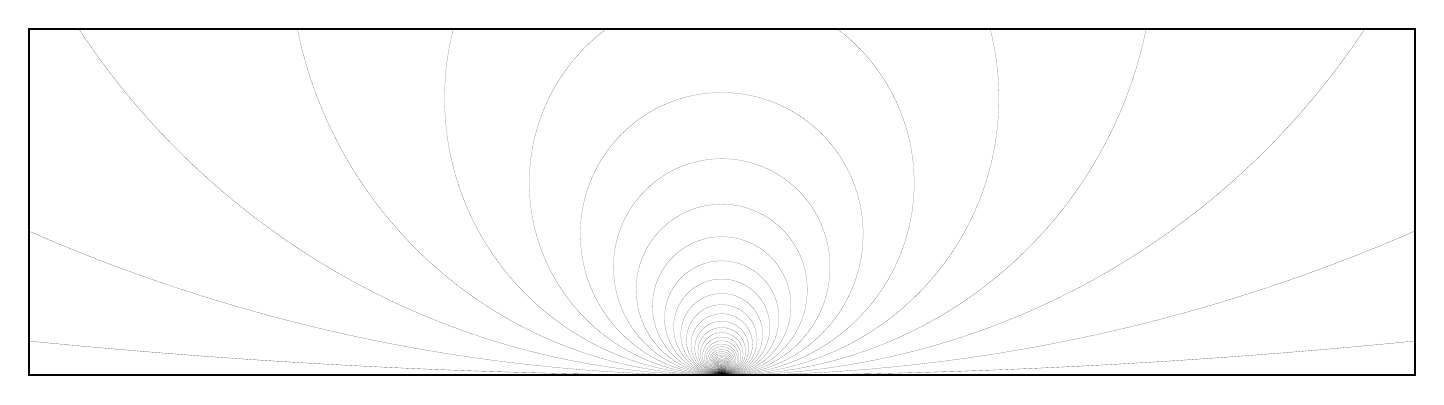
\begin{tikzpicture}[scale=88]
	\draw[thick] (-.1,0) rectangle (.1,.05);
	\clip (-.1,0) rectangle (.1,.05); % remove for all circles
	\foreach \i in {1,...,100}{
		\draw[line width=0.1/\i mm] (0, 1/\i^2) circle (1/\i^2);
	}
	\end{tikzpicture}
	\caption{TBW}
	\label{fig:earrings}
\end{figure}

In this section we show that a sublevel filtration can be $\HLC$ and not q-tame.

The $d$-dimensional Hawaiian earring is defined as the subspace
\begin{equation*}
\HE = \bigcup_{n\in\mathbb{N}}\left\{(x_0,\dots,x_d)\in\R^{d+1}\mid \left(x_0-\frac{1}{n}\right)^2+x_1^2+\dots+x_d^2=\left(\frac{1}{n}\right)^2\right\}
\end{equation*}
of $d+1$-dimensional Euclidean space.
Let $f \colon \HE\to\R$ as $0$ at the origin $\vec{0}$ and $1$ everywhere else.
All sublevel sets $\HE_{\leq t}$ are either the singleton $\{\vec{0}\}$ or the whole space $\HE$, and therefore compact.
Moreover, $\HE$ is locally-$f$-connected as we prove now. 

Let $e > 0$ and $p \in \HE$.
If $p$ is the origin, we choose $\delta$ between 0 and $\min\{e,1\}$.
Then $\HE_{\leq f(p) + \delta} = \HE_{\leq \delta} = \{p\}$, so the condition is trivially satisfied.
For $p$ not the origin, there is a unique $d$-sphere that contains it.
Clearly, we may choose $\delta$ so small that $B_{\delta}(p)$ contained in this sphere, so $B_{\delta}(p)$ is a disk and the condition follows trivially again. 

What remains to be shown is that $\HE_{\leq \bullet}$ is not q-tame with respect to singular and \v{C}ech homology.
Note that $\HE_{\leq t}$ is constant with value $\HE$ for $t \geq 1$, so it suffices to show that the singular and \v{C}ech homology of $\HE$ with field coefficients is infinite dimensional.
The case of singular homology is well know.
For \v{C}ech homology we use the fact that it commutes with inverse limits for compact Hausdorff spaces.
Define 
\begin{align*}
\HE_k &= \left\{(x_0,\dots,x_d)\in\R^{d+1}\mid \left(x_0-\frac{1}{k}\right)^2+x_1^2+\dots+x_d^2=\left(\frac{1}{k}\right)^2\right\}\\
&\cup\bigcup_{n=1}^{k-1}\left\{(x_0,\dots,x_d)\in\R^{d+1}\mid \left(x_0-\frac{1}{n}\right)^2+x_1^2+\dots+x_d^2=\left(\frac{1}{n}\right)^2\right\},
\end{align*}
i.e., the $d$-dimensional Hawaiian earring but with the $k$-th largest $d$-sphere filled.
We have $\lim_{k}\HE_{k} = \bigcap_{k}\mathbb{H}^{d}_{k}=\mathbb{H}^{d}$, and hence $\CH_{d}(\HE) = \lim_{k}\CH_{d}(\mathbb{H}^{d}_{k})$.
One can easily check that each $\mathbb{H}^{d}_{k}$ satisfies the assumptions for \cref{prop:cech_sing_hom_hlc}, which implies $\lim_{k}\CH_{d}(\mathbb{H}^{d}_{k})=\lim_{k}H_{d}(\mathbb{H}^{d}_{k})$.
We compute
\[
\lim_{k}H_{d}(\mathbb{H}^{d}_{k})=\lim\left(\dots\to \prod_{n=1}^2\mathbb{F}\to \prod_{n=1}^1\mathbb{F}\to \prod_{n=1}^0\mathbb{F}\right)=\prod_{n\in\mathbb{N}}\mathbb{F},
\]
which is infinite-dimensional over $\mathbb{F}$.
This finishes the proof.

\begin{rem}
Note that the singular persistent homology of the sublevel set filtration of $F$ above is also not q-tame because the $d$-dimensional Hawaiian earring has infinite-dimensional $d$-th singular homology \cite{Barratt.1962}. 
\end{rem}

\begin{rem}
The construction above does not yield a counterexample to \cref{con:q-tame_pers_cech_hom} because $\mathbb{H}^{d}$ is not strongly locally-$F$-connected at the origin.
\end{rem}

\section{Theorem} \label{sec:theorem}

In this section we introduce a stronger version of $\HLC$ for sublevel filtrations, and we show that Morse filtrations with this property are q-tame.

\begin{defi}
	A sublevel filtration $(X,f)$ is said to be \textit{strongly} $\HLC$ if for each $x \in X$, neighborhood $V$ of $x$ and $\epsilon > 0$ there exists $U$ a neighborhood of $x$ with $U \subseteq V$ and $\delta \in (0, \epsilon)$ such that
	\begin{equation*}
	X_{\leq f(x) + \delta + c} \cap U \to X_{f(x) + \epsilon + c} \cap V
	\end{equation*}
	is $\HT$ for every $c \geq 0$.
\end{defi}

\begin{thm} \label{t:strong local connectenss implies q-tameness}
	Any be a strongly $\HLC$ Morse filtration $(X,f)$ is q-tame, i.e., for every $s < t$ the inclusion $X_s \to X_t$ is $\HS$.
\end{thm}

\begin{lem} \label{l:commutative algebra}
	Given a commutative diagram of modules over a principal ideal domain
	\begin{equation*}
	\begin{tikzcd}
	A_{1,1} \arrow[r] & A_{1,2} & \\
	A_{2,1} \arrow[r] \arrow[u] & A_{2,2} \arrow[r] \arrow[u] & A_{2,3} \\
	& A_{3,2} \arrow[r] \arrow[u] & A_{3,3} \arrow[u]
	\end{tikzcd}
	\end{equation*}
	where the middle row is exact and both $A_{2,1} \to A_{1,1}$ and $A_{3,3} \to A_{2,3}$ have finitely generated images, then $A_{3,2} \to A_{1,2}$ does as well.
\end{lem}

\begin{proof}
	This is proven via a straightforward diagram chase. For complete details see Lemma 17.3 in \cite{Bredon.1968}.
\end{proof}

\begin{lem} \label{l:neighborhood third}
	Let $X$ be locally compact space.
	For any compact subset $K$ and open set $U$ with $K \subseteq U$ there exists a compact set $K^\prime$ such that
	\begin{equation*}
	K \subseteq \interior(K^\prime) \subseteq K^\prime \subseteq U.
	\end{equation*}
\end{lem}

\begin{proof}
	For any $x \in K$ choose a compact neighborhood $C(x) \subseteq U$.
	We have
	\begin{equation*}
	K \subseteq \bigcup_K \interior(C(x)) \subseteq \interior\left(\bigcup_K C(x)\right) \subseteq \bigcup_K C(x) \subseteq U
	\end{equation*}
	Since $K$ is compact, the first inclusion above is achieved over a finite subset $\{x_1, \dots, x_m\}$ of elements in $K$.
	Defining $K^\prime = \bigcup_{i=1}^m C(x_i)$ finishes the proof.
\end{proof}

\begin{lem} \label{l:key lemma for q-tameness}
	Fix a homology theory. Let $M$ and $f$ be as in Theorem \ref{t:strong local connectenss implies q-tameness}.
	Consider sets $K, L \subseteq M$ with $K$ compact and $K \subseteq \interior(L)$. For any $s < t$ there is $\delta \in (0,\, t-s)$ such that $K \cap M_{s+\delta} \to L \cap M_{t}$ is $\HS$.
\end{lem}

\begin{proof}
	The lemma holds for $\HS$ replaced by $\HS_{(n-1)}$ for any $n \leq 0$ since $H_{n-1}(-)$ induces the zero map. We will proceed by induction on $n$ assuming the lemma for $\HS_{(n-1)}$. 
	
	Given a compact set $L \subseteq M$ and $s < t$ let $\Sigma_{s, t}$ be the collection of all compact subsets $K$ of $\interior(L)$ for which there exists $\delta_K > 0$ and an open neighborhood $U_K$ of $K$ such that $U_K \cap M_{s+\delta_K} \to L \cap M_{t}$ is $\HS_n$.
	
	We start by showing that any point in $\interior(L) \cap M_s$ has a neighborhood in $\Sigma_{s, t}$.
	Let $x \in \interior(L) \cap M_{s}$ and take $e > 0$ such that $s + e < t$ and $B_e(x) \subseteq \interior(L)$.
	By the strong local-$f$-connectivity of $M$, there exists $\delta \in (0, e)$ such that for $c = s - f(x)$ the following composition is $\HS$:
	\begin{equation*}
	\overline B_{\delta/2}(x) \cap M_{s + \delta} \to
	B_\delta(x) \cap M_{s + \delta} =
	B_\delta(x) \cap M_{f(x) + c + \delta} \to
	B_e(x) \cap M_{f(x) + c + e} \to
	L \cap M_{t}.
	\end{equation*}  
	
	We will now show that the class $\Sigma_{s,t}$ is closed under finite unions.
	For $i \in \{1, 2\}$ let $K_i$ be in $\Sigma_{s,t}$ with $\delta_i > 0$ and $K_i \subseteq U_i$ open such that $U_{i} \cap M_{s+\delta_i} \to L \cap M_{t}$ is $\HS_n$.
	We Use Lemma \ref{l:neighborhood third} to construct sets $K_i^\prime$ such that
	\begin{equation*}
	K_i \subseteq \interior(K_i^\prime) \subseteq K_i^\prime \subseteq U_i.
	\end{equation*}
	Notice that for $\delta = \min(\delta_i)$ we have $K_i^\prime \cap M_{s+\delta} \to L \cap M_t$ is $\HS_n$.
	Additionally, the induction hypothesis implies that $K_1 \cap K_2 \cap M_s \to K_1^\prime \cap K_2^\prime \cap M_{s+\delta}$ is $\HS_{(n-1)}$.
	We therefore have the following commutative diagram satisfying the assumptions of Lemma~\ref{l:commutative algebra}:
	\begin{equation*}
	\begin{tikzcd}
	\H_n(L \cap M_t) \oplus \H_n(L \cap M_t) \arrow[r] &
	\H_n(L \cap M_t) & \\
	\H_{n}(K_1^\prime \cap M_{s+\delta}) \oplus \H_n(K_2^\prime \cap M_{s+\delta}) \arrow[r] \arrow[u] & 
	\H_{n}((K_1^\prime \cap M_{s+\delta}) \cup (K_2^\prime \cap M_{s+\delta})) \arrow[r] \arrow[u] &
	\H_{n-1}(K_1^\prime \cap K_2^\prime \cap M_{s+\delta}) \\ & 
	\H_{n}((K_1 \cup K_2) \cap M_s) \arrow[r] \arrow[u] &
	\H_{n-1}(K_1 \cap K_2 \cap M_s). \arrow[u]
	\end{tikzcd}
	\end{equation*}
	We conclude that $K_1 \cup K_2 \in \Sigma_{s, t}$.
	Since any compact $K \subseteq \interior(L)$ can be expressed as a finite union of sets in $\Sigma_{s,t}$ the induction step and the lemma are proven.
\end{proof}

\begin{proof}[Proof of Theorem \ref{t:strong local connectenss implies q-tameness}]
	It follows from applying Lemma~\ref{l:key lemma for q-tameness} to $K = M_{\leq s}$ and $L = M$.
\end{proof}
\input{outlook}
%
\subsection{Two Alternative Conjectures}
In order to relate Morse's conditions to the above, we need a relative version of the $HLC^{\infty}$ condition.

\begin{defi}\label{defi:hlc}
Let $\mathcal{C}$ be a category with $0$ object and let $A\colon\mathbf{Top}\to\mathcal{C}$ be a functor. If $Y\subseteq X$ is a pair of topological spaces, we say that $Y$ is \emph{locally connected with respect to $A$ in $X$} if for each point $p\in Y$ and any open neighborhood $V$ of $p$ in $X$ there is an open neighborhood $U\subseteq V$ of $p$ such that $A(U\cap Y\hookrightarrow V)$ factors through 0.

We say that $Y$ is \emph{$HLC^{\infty}$ in $X$} if it is locally connected with respect to $\tilde{H}_*(-;\mathbb{Z})$ in $X$.
\end{defi}

We get the following rephrasing of strong local-$f$-connectedness.

\begin{prop}
Let $M$ be a metric space and $f\colon M\to\mathbb{R}$ a function. Then $M$ is strongly locally-$f$-connected if and only if $f_{\leq s}$ is $HLC^{\infty}$ in $f_{\leq t}$ whenever $s<t$.
\end{prop}
\begin{proof}
If each sublevel set is $HLC^{\infty}$ in larger sublevel sets, $M$ is clearly strongly locally-$f$-connected. For the converse direction, fix $s<t$ and choose some point $p\in f_{\leq s}$ with a neighborhood $V$ of $p$ in $f_{\leq t}$. We may choose $e\in(0, t-s)$ such that $B_e(p)\cap f_{\leq t}\subseteq V$. By strong local-$f$-connectedness, for each $d$ there is some $\delta\in(0,e)$ such that the map in reduced $d$-dimensional homology induced by $B_{\delta}(p)\cap f_{\leq s}\hookrightarrow B_e(p)\cap f_{\leq t}$ is trivial. The map $B_{\delta}(p)\cap f_{\leq s}\hookrightarrow V$ factors through the aforementioned map, so it is trivial in reduced homology, too. Thus, $f_{\leq s}$ is $HLC^{\infty}$ in $f_{\leq t}$.
\end{proof}

Note that the proposition gives a purely topological description of strong local-$f$-connectedness, so we can also use it to define strong local-$f$-connectedness for spaces that are not metrizable. It also yields the following corollary.

\begin{cor}
Let $M$ be a topological space and $f\colon M\to\mathbb{R}$ a function. If all sublevel sets are $HLC^{\infty}$, then $M$ is strongly locally-$f$-connected.
\end{cor}

We now propose the following generalization of \cref{prop:fin_dim_sing_hom}.

\begin{conj}\label{conj:q-tame_singular}
Let $Y\subseteq X$ be compact Hausdorff spaces such that $Y$ is $HLC^{\infty}$ in $X$. Then $\im H_d(Y\hookrightarrow X)$ is finite-dimensional for all $d$.
\end{conj}

As a persistent version, we have the following obvious consequence.

\begin{prop}\label{prop:q-tame_singular}
Let $M$ be a topological space and $f\colon M\to\mathbb{R}$ a function such that $M$ is strongly locally-$f$-connected, i.e., each sublevel set is $HLC^{\infty}$ in all larger sublevel sets. If \cref{conj:q-tame_singular} is true, then $H_{d}(f_{\leq\bullet})$ is q-tame for all $d$.
\end{prop}

In a similar spirit, we also propose the following conjecture as an analogue to \cref{cor:cech_sing_persistent_iso}.

\begin{conj}\label{con:d_I_0_sing_cech}
Let $M$ be a topological space and $f\colon M\to\mathbb{R}$ a function such that all sublevel sets are paracompact Hausdorff. If $M$ is strongly locally-$f$-connected, i.e., each sublevel set is $HLC^{\infty}$ in all larger sublevel sets, then 
\[
d_I(H_d(f_{\leq\bullet}),\CH_d(f_{\leq\bullet}))=0
\]
for all $d$.
\end{conj}

Here, $d_{I}$ denotes the interleaving distance between persistence modules. The conjecture is relevant because of the following criterion for q-tameness.

\begin{prop}
Let $M$ and $N$ be persistence modules such that $M$ is q-tame and assume $d_I(M,N)=0$. Then $N$ is q-tame.
\end{prop}
\begin{proof}
Pick indices $s<t$. Because $d_I(M,N)=0$, we may choose a $\delta$-interleaving with $\delta\in\left(0,\frac{t-s}{2}\right)$. Then we have a commutative diagram 

\[
\begin{tikzcd}
N_s\arrow[rrr]\arrow[rd]&&&N_{t}\\
&M_{s+\delta}\arrow[r]&M_{t-\delta}\arrow[ru]&
\end{tikzcd}
\]
so that the rank of $N_s\to N_t$ is bounded above by the rank of $M_{s+\delta}\to M_{t-\delta}$. The rank of $M_{s+\delta}\to M_{t-\delta}$ is finite by assumption, so $N$ is q-tame.
\end{proof}

Combining the previous result with \cref{prop:q-tame_singular}, we get the following.

\begin{cor}
If \cref{conj:q-tame_singular,con:d_I_0_sing_cech} are true, then so is \cref{con:q-tame_pers_cech_hom}.
\end{cor}

Thus, we have reduced our main conjecture to two smaller ones.

A possible proof strategy for \cref{conj:q-tame_singular} might be to adapt the proof strategy of Wilder's Finiteness Theorem, which is an analogue of \cref{prop:fin_dim_sing_hom} for sheaf cohomology, from \cite[Section II.17]{MR1481706}. Essentially the same proof also appears in \cite[Section III.10]{MR842190}.

A possible proof strategy for \cref{con:d_I_0_sing_cech} might be to adapt Bredon's proof of \cref{prop:cech_sing_hom_hlc} using his spectral sequence that relates \v{C}ech and singular homology.

\subsection{Q-Tameness of Persistent \v{C}ech Homology via Cosheaf Homology}\label{sec:cosheaf}
Note that what follows is rather informal and speculative.

When working with cohomology, the usual modern way to relate the singular and the \v{C}ech theory is via an intermediate step in the form of sheaf cohomology and then use the Leray and Grothendieck spectral sequences \cite[Chapter III]{MR1481706}. One might hope to use similar cosheaf theoretic methods, such as a possible theory of cosheaf homology, to obtain similar results for homology. So far, treatments of cosheaf homology are sparse. Among them are \cite{Andreotti.1973}, \cite{Schneiders.1987} and \cite{prasolov2018cosheaves}, but we are presently unable to determine whether the techniques in these texts can be adapted to our problems. Bredon, in \cite{Bredon.1968} and \cite[Chapter VI]{MR1481706}, also defines \v{C}ech homology with coefficients in a precosheaf and compares it to the singular theory for paracompact $HLC^{\infty}$-spaces \cite[Section VI.4 and Theorem VI.12.6]{MR1481706} using cosheaf theoretic methods. All of his results are still absolute comparison and finiteness results, i.e., they work for a single space $X$, so another obstacle, besides cosheaf homology being underdeveloped, is our desired generalization to subspaces $Y\subseteq X$ that are only $HLC^{\infty}$ in $X$ but not in themselves. That cosheaves might also help in overcoming this problem is suggested by the very nice formulation of the $HLC^{\infty}$ property in terms of precosheaves. The following definition appears in \cite{MR1481706}.

\begin{defi}
Let $\mathfrak{A}$ be a precosheaf on a space $X$ with values in a category with 0 object, i.e., a covariant functor on the poset category of open sets in $X$. We call $\mathfrak{A}$ \emph{locally trivial} if for all points $x\in X$ and all open neighborhoods $V$ of $x$ there is another open neighborhood $U\subseteq V$ of $x$ such that $\mathfrak{A}(U)\to\mathfrak{A}(V)$ factors through 0.
\end{defi}

The following definition is, up to our use of reduced homology, taken from \cite{Curry.2015}.

\begin{defi}
For any topological space $X$, we define the \emph{reduced Leray precosheaf} $\mathfrak{L}_X$ on $X$ as the precosheaf mapping $U\mapsto \tilde{H}_*(U;\mathbb{Z})$.
\end{defi}

\begin{defi}
If $f\colon Y\to X$ is a continuous map between topological spaces and $\mathfrak{A}$ is a precosheaf on $Y$, we define the \emph{pushforward of $\mathfrak{A}$ along $f$} as the precosheaf on $X$ mapping $U\mapsto\mathfrak{A}(f^{-1}(U))$. We denote it by $f_*\mathfrak{A}$.
\end{defi}

Now if $Y\subseteq X$ are topological spaces, we get an obvious morphism $i_*\mathfrak{L}_Y\to\mathfrak{L}_X$ of precosheaves on $X$, where $i\colon Y\hookrightarrow X$ is the inclusion, given by $\tilde{H}_*(U\cap Y\hookrightarrow U;\mathbb{Z})$. Note that the category of precosheaves with values in abelian groups is just a functor category from a small category to an abelian category. In particular, it has images given "pointwise". We get the following rephrasing of the relative $HLC^{\infty}$ property.

\begin{prop}
Let $Y\subseteq X$ be topological spaces. Then $Y$ is $HLC^{\infty}$ in $X$ if and only if $\im(i_*\mathfrak{L}_Y\to\mathfrak{L}_X)$ is locally trivial.
\end{prop}

Our hope is that one might be able to use this characterization in the future to prove the previously made conjectures.

\todo{Given $f\colon M\to\mathbb{R}$, is there a way of finding a single space (e.g. M itself, disjoint union of sublevel sets, colim of sublevel sets, hocolim of sublevel sets, continuously indexed mapping telescope (how to construct this?) of inclusions of sublevel sets, etc.) and a precosheaf with values in a category of persistence module (maybe the observable category) on that space such that $M$ is locally-$f$-connected iff that precosheaf is locally trivial?}

\section*{Acknowledgements}
This research has been supported by German Research Foundation (DFG) through the Collaborative Research Center SFB/TRR 109 \emph{Discretization in Geometry and Dynamics}, the Collaborative Research Center SFB/TRR 191 \emph{Symplectic Structures in Geometry, Algebra and Dynamics}, the Cluster of Excellence EXC-2181/1 \emph{STRUCTURES}, and the Research Training Group RTG 2229 \emph{Asymptotic Invariants and Limits of Groups and Spaces}.

\bibliographystyle{abbrvnaturl}
\bibliography{biblio}

\todos
\end{document}